\documentclass[portrait,final,a0paper,fontscale=0.31]{baposter}

%% read in constants, custom functions and used packages

%%%%%%%%%%%%%%%%%%%%%%%%%%%%%%%%%%%%%%%%%%%%%%%%%%%%%%%%%%%%%%%%%%%%%%%% References paths
\usepackage[backend=biber, style=apa, citestyle=apa]{biblatex}
\addbibresource{refs.bib}
\AtBeginBibliography{\small}

%%%%%%%%%%%%%%%%%%%%%%%%%%%%%%%%%%%%%%%%%%%%%%%%%%%%%%%%%%%%%%%%%%%%%%%% Image paths
\usepackage{graphicx}
\graphicspath{{logos/}{figures/}}

%%%%%%%%%%%%%%%%%%%%%%%%%%%%%%%%%%%%%%%%%%%%%%%%%%%%%%%%%%%%%%%%%%%%%%%% Color Settings
\usepackage{xcolor}
\definecolor{iftucfont}{RGB}{74,130,70}
\definecolor{iftuccolor}{RGB}{143,168,92}
\definecolor{iftucbackground}{RGB}{241,244,234}

%%%%%%%%%%%%%%%%%%%%%%%%%%%%%%%%%%%%%%%%%%%%%%%%%%%%%%%%%%%%%%%%%%%%%%%% Font Settings
\usepackage[sfdefault, regular]{roboto}

%%%%%%%%%%%%%%%%%%%%%%%%%%%%%%%%%%%%%%%%%%%%%%%%%%%%%%%%%%%%%%%%%%%%%%%% Multicol Settings
\usepackage{multirow}
\usepackage{multicol}
\setlength{\columnsep}{1.5em}
\setlength{\columnseprule}{0mm}

%% Row Settings
\usepackage{setspace}% for \onehalfspacing
\usepackage{parskip}

%% Control layout of itemize, enumerate, description
\usepackage{enumitem}

% page borders and header height
\usepackage{geometry}
\geometry{
	left=35pt,
	right=5pt,
	top=10pt
}

\newcommand{\compresslist}{% Define a command to reduce spacing within itemize/enumerate environments, e.g. \begin{itemize}\compresslist
			\setlength{\itemsep}{1pt}
			\setlength{\parskip}{0pt}
			\setlength{\parsep}{0pt}
		}
	
\newcommand{\compressbib}{%
		\setlength{\itemsep}{0pt}
		\setlength{\parskip}{0pt}
		\setlength{\parsep}{0pt}}
	
%%%%%%%%%%%%%%%%%%%%%%%%%%%%%%%%%%%%%%%%%%%%%%%%%%%%%%%%%%%%%%%%%%%%%%%% Table and figure settings
\usepackage{float, booktabs,array}

% Adjust row width in tables 
\renewcommand{\arraystretch}{1.1}

% for awesome plots and tables from files like .csv
\usepackage{pgfplots}
\usepackage{pgfplotstable}

% Graphics package-alike macros for “general” boxes. Like resizing figures and aligning minipages
\usepackage{adjustbox}

\usepackage[
font=footnotesize,
labelfont=bf,
%labelfont=sc, %Kapitälchen, passt nicht wg. nicht-osf Ziffern
%%%%labelfont=it, %italics, 
%%%labelfont=sl, %slanted,
hypcap=true,
format=hang,
%margin={2cm,2cm}
width=0.8\linewidth
]{caption}

%%%%%%%%%%%%%%%%%%%%%%%%%%%%%%%%%%%%%%%%%%%%%%%%%%%%%%%%%%%%%%%%%%%%%%%% Other packages
% to help with long equations
\usepackage{amsmath}

% for todo notes
\usepackage{todonotes} 

% for comment blocks
\usepackage{verbatim}

% link URLs
\usepackage{url}

\usepackage{lipsum}


\begin{document}

\begin{poster}%
	% Poster Options
	{
		% Show grid to help with alignment
		grid=false,
		% Number of columns and column spacing
		columns=6,
		colspacing=1em,
		% Color style
		bgColorOne=white,
		borderColor=iftuccolor,
		headerColorOne=iftucbackground,
		headerFontColor=iftucfont,
		boxColorOne=white,
		% Format of textbox
		textborder=rounded,
		textfont=\small,
		% Format of text header
		eyecatcher=true,
		headerborder=closed,
		headerheight=0.1\textheight,
		%  textfont=\sc, An example of changing the text font
		headershape=rounded,
		headershade=plain,
		headerfont=\Large\bf, %Sans Serif
		% textfont={\setlength{\parindent}{1.5em}},
		boxshade=plain,
		%  background=shade-tb,
		background=plain,
		linewidth=2pt
	}
	% University logo
	{
\includegraphics[height=6.5em]{tuckhseng_color}} 
	% Title
	{\bf\Large{Dynamic and adaptive body schema by learning to predict the sensory consequences of actions}\vspace{1em}}
	% Authors
	{\large Erik~Syniawa\textsuperscript{2}, Valentin~Forch\textsuperscript{1} and Fred~Hamker \\ \vspace{0.5em}
	\small Contact: erik.syniawa@informatik.tu-chemnitz.de
	}
	% Department logo and other logos
	{	
		\begin{minipage}[r]{0.1\textwidth}
			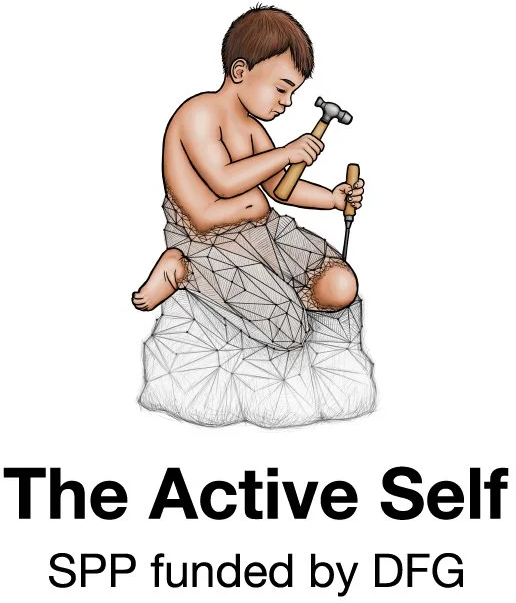
\includegraphics[height=7em]{active_self_logo_color}
		\end{minipage}
		\hfill
		\begin{minipage}[r]{0.1\textwidth}
			
\includegraphics[height=6.5em]{TUC_AI_color}
		\end{minipage}
		
	}

%%%%%%%%%%%%%%%%%%%%%%%%%%%%%%%%%%%%%%%%%%%%%%%%%%%%%%%%%%%%%%%%%%
% use height in headerbox to align multiple boxes 
% height= <size in percent of column height>, else [auto]%
\headerbox{Overview}{name=overview,column=0,row=0, span=6}{
	
	
	\begin{adjustbox}{minipage=0.95\textwidth, margin=5pt, center}
	Systems-level approach to develop a body schema and agency:
	
	\begin{minipage}[r]{0.6\textwidth}
		\begin{itemize}
		\item The \textbf{basal ganglia} will select an action based on the desired state (see \cite{baladronHabitLearningHierarchical2020}).
		\item The \textbf{central pattern generator} will be execute the action (see \cite{nassourConcreteActionRepresentation2020}).
		\item The \textbf{cerebellum} will learn to predict the sensory consequences of the motor action in all modalities (vision, touch, proprioception) i.e. the body schema (see \cite{schmidForwardModelsCerebellum2019}). 
		\item The \textbf{prediction error} will be used to improve the prediction and to train action selection in the \textbf{basal ganglia}.
		\end{itemize}
	\end{minipage}
	\begin{minipage}[r]{0.1\textwidth}
	\end{minipage}
	\begin{minipage}[l]{0.4\textwidth}
		\raggedleft
		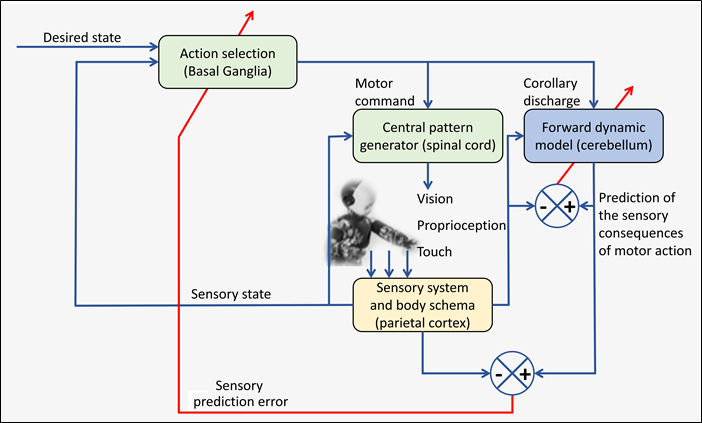
\includegraphics[width=0.8\linewidth]{model}
		\captionof{figure}{babbas}
	\end{minipage}
	\end{adjustbox}
	
	\vspace{0.3em}
}

\headerbox{\large Recurrent Basis Functions\textsuperscript{1}}{name=rbf, column=0, below=overview, span=2, height=0.3}{
	
	\begin{adjustbox}{minipage=0.95\textwidth, margin=5pt, center}
		Hier was zu dieser Veröffentlichung \cite{pougetComputationalPerspectiveNeural2002}.
	
		\vspace{0.3em}
		\begin{center}
			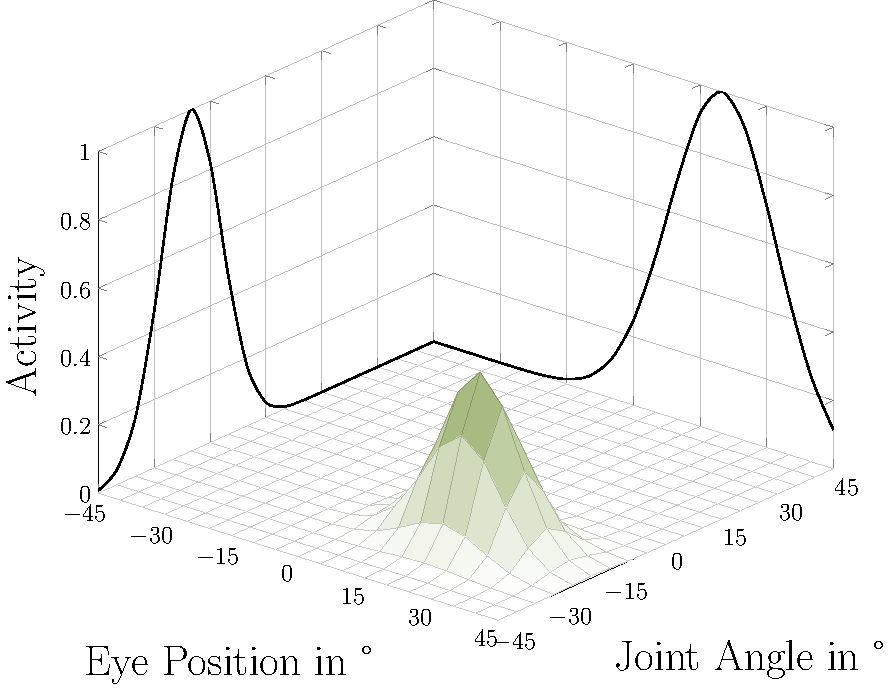
\includegraphics[width=0.9\linewidth]{pop_code_figure}
			\captionof{figure}{babbas}
		\end{center}
	\end{adjustbox}
}

\headerbox{\large Learning a Body Schema\textsuperscript{1}}{name=network, column=2, below=overview, span=4, height=0.3}{
	\begin{adjustbox}{minipage=0.95\textwidth, margin=5pt, center}

	\end{adjustbox}
}

\headerbox{\large References}{name=refs, column=0, above=bottom, span=6}{
	\begin{adjustbox}{minipage=0.98\textwidth, margin=0pt, center}
		
		\compressbib{\printbibliography[heading=none]}
		
		
	\end{adjustbox}
	
	
}

\headerbox{\large Basal Ganglia\textsuperscript{2}}{name=bg, column=0, below=rbf, above=refs , span=3}{
	\begin{adjustbox}{minipage=0.95\textwidth, margin=5pt, center}
		
		\begin{minipage}[t]{\textwidth}
			\footnotesize
			\begin{multicols}{2}
			The 3-factor learning principles are primarily determined by presynaptic and postsynaptic neuron activity, as well as the dopamine signal. \\
			The labels high and low indicate whether the pre- and post-activity is more than or less than a given threshold (for example, mean population activity). \\
			DA+ and DA- labels indicate if SNc activity is above or below a given threshold. A sign specifies the weight changes in the relevant projections for each combination of these criteria (+,, no sign). Table S8 contains the real mathematical explanation of plasticity, in addition to the general description offered. 
			\end{multicols}
			\vspace{2pt}
		\end{minipage}
		\hfill
	
		\begin{minipage}[r]{0.48\textwidth}
			\raggedleft
			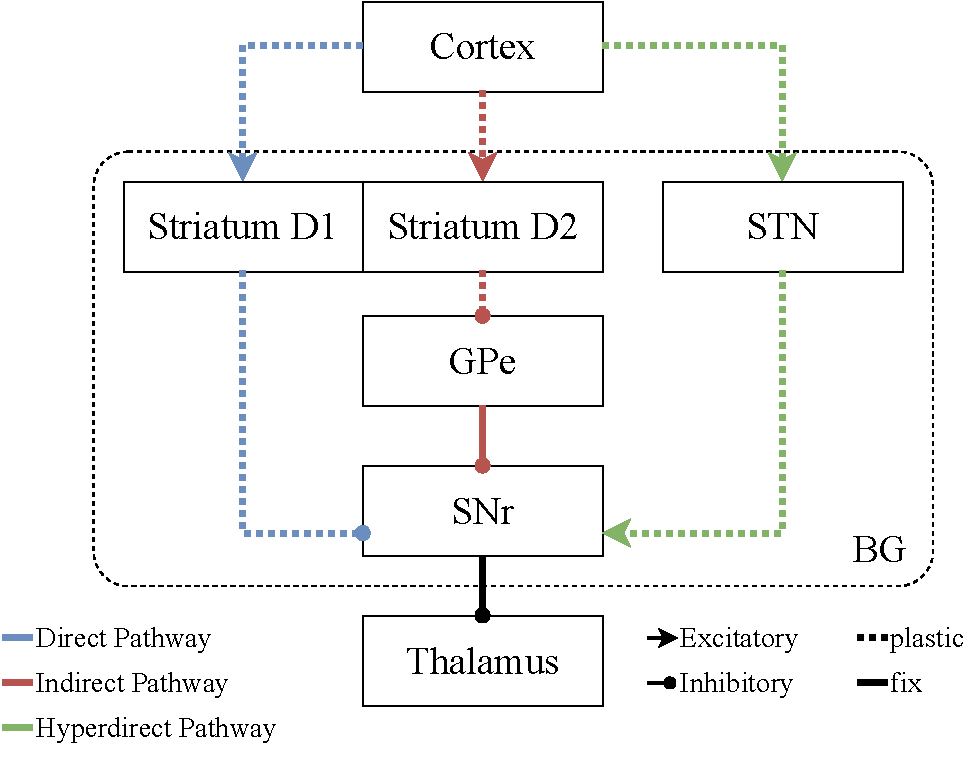
\includegraphics[width=\linewidth]{BGresize}
			\captionof{figure}{Modeling of segregated \\ basal ganglia pathways}
		\end{minipage}
		\hfill
		\begin{minipage}[l]{0.49\textwidth}
			\resizebox{\columnwidth}{!}{%
	\begin{tabular}{lcccccl}
		\multicolumn{2}{l}{\multirow{4}{*}{}}          & \multicolumn{4}{c}{\textbf{Dopamine}}               & \multirow{4}{*}{}                    \\ \cline{3-6}
		\multicolumn{2}{l}{}                           & \multicolumn{2}{c}{DA +} & \multicolumn{2}{c}{DA -} &                                      \\ \cline{3-6}
		\multicolumn{2}{l}{}                           & \multicolumn{4}{c}{\textbf{Post-activity}}          &                                      \\ \cline{3-6}
		\multicolumn{2}{l}{}                           & High        & Low        & High        & Low        &                                      \\ \hline
		\multirow{12}{*}{\textbf{Pre-activity}} & High & +           &            & -           &            & \multirow{2}{*}{\textbf{Cortex-D1}}  \\
		& Low  & -           &            &             &            &                                      \\ \cline{2-7} 
		& High & -           &            & +           &            & \multirow{2}{*}{\textbf{Cortex-D2}}  \\
		& Low  &             &            & -           &            &                                      \\ \cline{2-7} 
		& High & +           &            & -           &            & \multirow{2}{*}{\textbf{Cortex-STN}} \\
		& Low  & -           &            &             &            &                                      \\ \cline{2-7} 
		& High & -           & +          &             & -          & \multirow{2}{*}{\textbf{D1-SNr}}     \\
		& Low  &             &            &             &            &                                      \\ \cline{2-7} 
		& High &             & -          & -           & +          & \multirow{2}{*}{\textbf{D2-GPe}}     \\
		& Low  &             &            &             &            &                                      \\ \cline{2-7} 
		& High & +           & -          &             & +          & \multirow{2}{*}{\textbf{STN-SNr}}    \\
		& Low  &             &            &             &            &                                      \\ \hline
	\end{tabular}
}
			\captionof{table}{+: LTP; -: LTD; \\ no sign: no weight change}
		\end{minipage}
	\end{adjustbox}

}

\headerbox{\large Motor Learning with the Basal Ganglia\textsuperscript{2}}{name=motor, column=3, below=network, above=refs , span=3}{
	
	\begin{minipage}[l]{0.35\textwidth}
		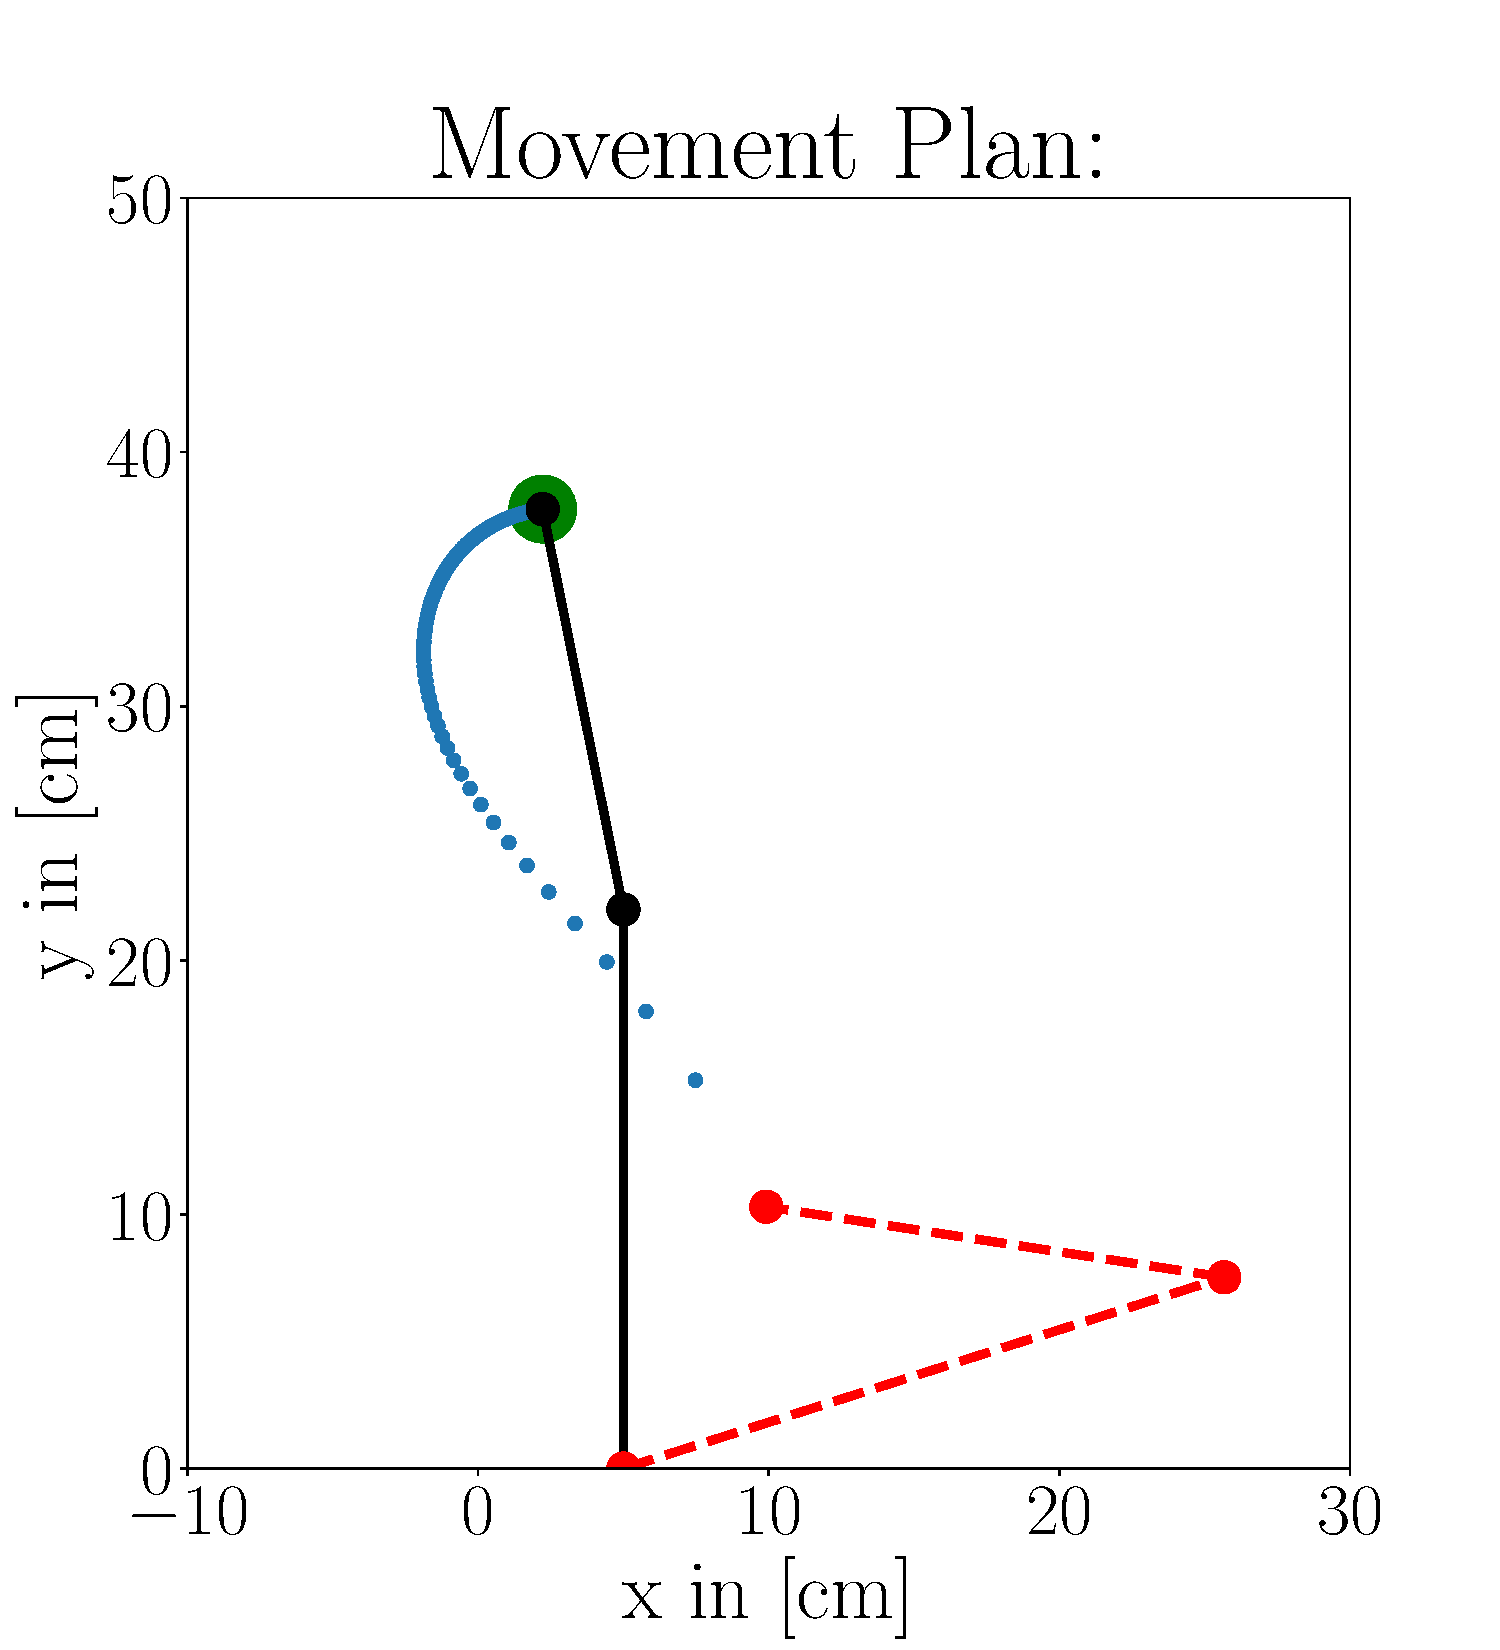
\includegraphics[width=0.9\linewidth]{movement}
		\vfill
		\captionof{figure}{Right: Development \\ of motor learning in the \\ different  pathways.}
	\end{minipage}
	\hfill
	\begin{minipage}[r]{0.65\textwidth}
		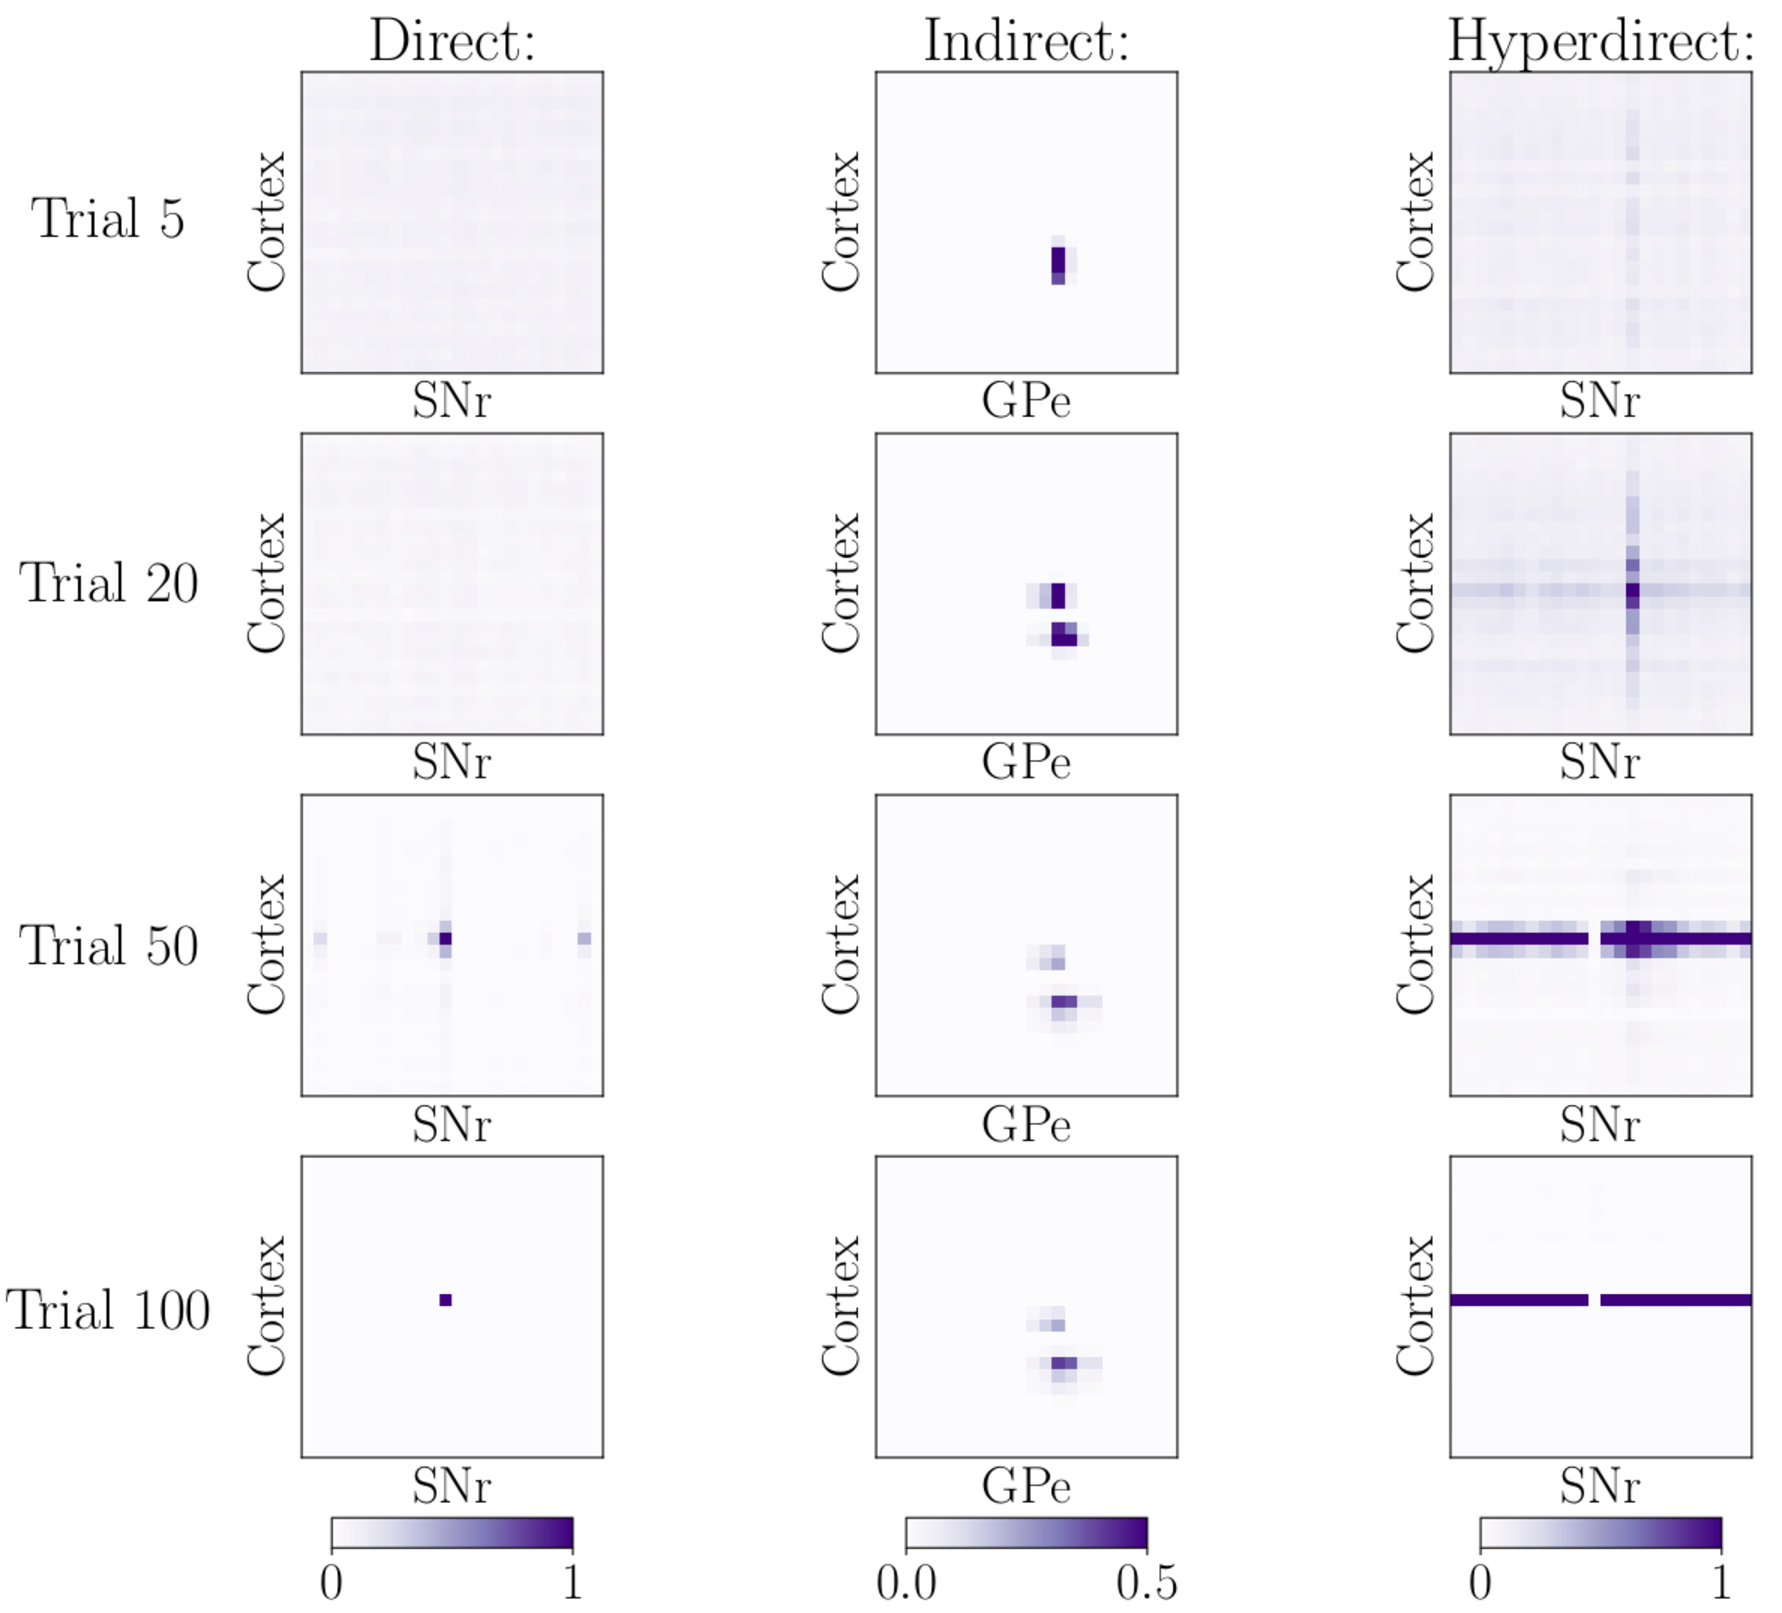
\includegraphics[width=\linewidth]{BG_Learning}
	\end{minipage}
	\begin{adjustbox}{minipage=0.95\textwidth, margin=5pt, center}
			
		\begin{minipage}[b]{\textwidth}
			\begin{multicols}{2}
			The 3-factor learning principles are primarily determined by presynaptic and postsynaptic neuron activity, as well as the dopamine signal. \\
			The labels high and low indicate whether the pre- and post-activity is more than or less than a given threshold (for example, mean population activity). \\
			DA+ and DA- labels indicate if SNc activity is above or below a given threshold. 
			\end{multicols}
		\end{minipage}
	
		
	\end{adjustbox}

	

}


\end{poster}


\end{document}